\section{Components of inertia matrix}
\label{app:inertia_sphere}
Let's recall equation~\myref{eq:component_inertia}.
\[ J_{\Delta} = \iiint d(u,\Delta)^2 \rho \dif V \]

Let's compute
\[ J_{zz} = \iiint d(u,Oz)^2 \rho \dif V \]
where $u$ is any point contained in the sphere.
In the case of the sphere, we have $J_{xx}=J_{yy}=J_{zz}$.

Using spherical coordinates $(r,\phi,\theta)$ for $x$
as shown in Figure~\ref{fig:sphere_coord}, this gives us
\[ 
  J_{zz} = \int_0^{2\pi} \dif \phi \int_0^{\pi} \dif \theta 
  \int_0^R (r \sin{\theta})^2 \rho\, r^2 \sin{\theta} \dif r
\]
the easy part
\[ 
  J_{zz} = \frac{2}{5} \rho\,\pi R^5 \int_0^{\pi} \sin^3{\theta} \dif \theta 
\]
the need-more-math part, knowing that
\[
  \int \sin^3{\theta} \dif \theta
  = \frac{1}{3} \cos^3{\theta} - \cos{x}
\] 
gives as expected
\[
  J_{zz} = \frac{2}{5} M R^2
\]

\begin{figure}[h]
  \begin{center}
    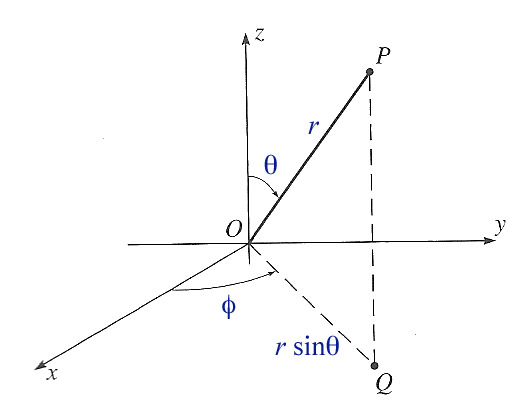
\includegraphics[scale=0.5]{spherical_coord.jpg}
    \caption{Spherical coordinates used 
    in Appendix~\ref{app:inertia_sphere}.}
    \label{fig:sphere_coord}
  \end{center}
\end{figure}

Another way to do it, is to slice up the solid sphere
into infinitesimally thin solid cylinders,
as shown in Figure~\ref{fig:moment_inertia_sphere}.
Knowing that the moment of inertia for a solid cylinder is 
\[ J_{zz} = \frac{1}{2}M R^2 \]
Applied to this problem we get
\[ \dif J_{zz} = \frac{1}{2} r^2 \dif m \]
where $\dif m = \rho \dif V$, and
\[ \dif V = \pi r^2 \dif x\]
we also notice that $r^2 = R^2 - x^2$, thus
\[ \dif J_{zz} = \frac{1}{2} \rho \, \pi (R^2 - x^2)^2 \dif x \]
We integrate over $[-R,R]$, which gives
\[ J_{zz} = \frac{8}{15} \rho \, \pi R^5 \]
Hence,
\[ \rho = \frac{M}{V} = \frac{M}{4/3 \pi R^3} \]
Finally,
\[ J_{zz} = \frac{2}{5} M R^2 \]

\begin{figure}
  \begin{center}
    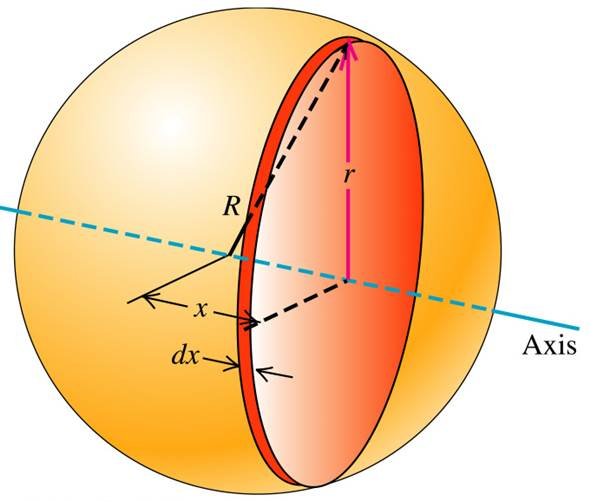
\includegraphics[scale=0.5]{moment_inertia_sphere.jpg}
    \caption{Scheme for computing the moment of inertia of
    a spherical rigid body of mass $M$ and radius $R$.}
    \label{fig:moment_inertia_sphere}
  \end{center}
\end{figure}